
\documentclass[12pt]{article}

\usepackage{sbc-template}

\usepackage{graphicx,url}

\usepackage[brazil]{babel}
\usepackage[utf8]{inputenc}  

     
\sloppy

\title{Algoritmos para o Problema do Caixeiro Viajante}

\author{Mateus Vitor Mota Vasconcelos\inst{1}}

\address{Universidade Federal de Minas Gerais
  \email{mateusvmv@ufmg.br}
}

\begin{document}

\maketitle

\begin{resumo} 
  Esse documento descreve duas implementações de algoritmos aproximativos para
  o problema do Caixeiro Viajante, os algoritmos Twice Around the Tree e
  o algoritmo de Christofides, bem como uma implementação de Branch and Bound,
  um algoritmo exaustivo e exato. As implementações foram comparadas em questão
  de qualidade da solução e tempo de execução, tanto com casos aleatórios de tamanho
  baixo quanto com problemas do conjunta TSPLIB.
  \footnote{Disponível em \url{https://github.com/mateusvmv/alg2_tsp}}
\end{resumo}

\section{Problema do Caixeiro Viajante}
Caixeiro Viajante é o nome de um problema NP-Difícil \cite{cormen2009introduction} que consiste em retornar
o caminho mais curto que passe por todos os pontos de um conjunto e retorne
para o ponto de início, como um caixeiro que deve vender suas mercadorias em
diversas cidades e retornar ao fim. É um problema difícil, e apenas em 1954
foi descoberta uma solução para 49 cidades, à mão, por \cite{dantzig1954solution}.

Por ser um problema NP-Dificil, não há solução polinomial para a melhor solução,
e o uso de algoritmos aproximativos é o único meio de se obter soluções de forma
eficiente. Como o problema tem usos práticos bastante comuns, há bastante interesse
em formas eficazes e eficientes de resolvê-lo.

\section{Algoritmo Twice Around the Tree}
O algoritmo Twice Around the Tree baseia-se em uma Árvore Geradora Mínima para
obter uma solução 2-aproximada para o problema do Caixeiro Viajante. O problema da
Árvore Geradora Mínima é similar ao Caixeiro Viajante, aqui queremos obter uma
árvore que atinja todos os vértices de um grafo com o menor peso nas arestas.
Enquanto o Caixeiro Viajante busca reduzir o custo da viajem pelas arestas na ida
e na volta, a Árvore Geradora reduz o custo das arestas sem o custo de retorno
\cite{rosenkrantz1977analysis}.

Para transformar a Árvore Geradora Mínima em uma solução para o Caixeiro Viajante,
o TATT percorre essa árvore com um Tour de Euler, e pula os vértices repetidos
para obter um Circuito Hamiltoniano. Por fim, o algoritmo apenas retorna ao começo.

O nome se dá pelo fato de que a árvore é percorrida duas vezes em cada aresta,
uma para proseguir e a outra para retornar. A Árvore Geradora Mínima é sempre
estritamente menor que a solução ótima para o Caixeiro Viajante, isso é porque
toda solução do Caixeiro Viajante, menos uma aresta qualquer, é uma Árvore Geradora.
Por isso, quando obtemos a árvore e percorremos cada aresta duas vezes, temos
um fator de aproximação de $O(2)$.

\section{Algoritmo de Christofides}
O algoritmo de Christofides \cite{christofides1976worst} baseia-se em uma ideia similar ao TATT, porém realiza
um passo a mais. Ao obter a Árvore Geradora Mínima, ela contém arestas de grau
ímpar, por isso não contém nenhum Tour como subgrafo. Para mudar isso, esse
algoritmo cria um Emparelhamento Mínimo dos nós de grau ímpar da Árvore Geradora,
e coloca as arestas do emparelhamento em um novo grafo. Esse grafo tem custo total
nas arestas igual ao custo das arestas da árvore, somado ao custo das arestas do
emparelhamento, e todos os vértices tem grau par.

Assim, é possível entrar e sair de qualquer vértice, e utilizando de um Tour
de Euler sem visitas repetidas, geramos um Circuito Hamiltoniano tal como no
TATT, e fechamos o circuito, obtendo uma solução para o Caixeiro Viajante.
Essa solução tem um custo limitado ao custo das arestas, e diferente do TATT,
no CF é possível retornar usando outras arestas do grafo, por isso
não dobramos o custo das arestas.

O fator de aproximação, então, é o valor da Árvore Geradora Mínima acrescido
do valor do Emparelhamento Mínimo. Como o valor da árvore é um limite inferior
para o valor da solução do Caixeiro Viajante, e como as arestas do
emparelhamento são limitadas pela metade do custo da árvore, a solução que o
algoritmo produz é uma aproximação com fator $O(3/2)$.

\section{Algoritmo Branch and Bound}
Diferente dos dois algoritmos anteriores, o algoritmo Branch and Bound não
produz soluções aproximadas, mas exatas. Ele baseia-se no fato de que é possível
obter um limite inferior e superior para uma solução do Caixeiro Viajante antes
mesmo de tê-la por completo, ao olhar para as arestas dos nós que ainda não tem
$grau=2$.

Para isso, definimos o limite inferior de uma solução como a soma da menor
aresta adjascente a cada vértice de $grau<2$ com a segunda menor aresta adjascente
a cada vértice de $grau<1$, dividido pela metade, e somado ao peso das arestas
que já estão inclusas na solução. Já o limite superior é semelhante, mas usa
as maiores arestas no lugar das menores.

O algoritmo prossegue como se fosse uma solução de força bruta, porém sempre
que adiciona uma aresta na recursão, observa os limites inferiores e superiores.
Se o limite inferior de uma solução é pelo menos o valor de algum outro limite
superior conhecido, não é preciso continuar o caminho atual. Assim, o algoritmo
corta grande parte dos caminhos ineficientes e é capaz de terminar mais rápido.

Para facilitar no corte de soluções ruins, o algoritmo já começa com uma solução
aproximativa, gerada pelo TATT ou pelo CF, como um limite superior, e também usa
da heurística de Depth First Search, que procura por soluções completas antes de
soluções que possam ter um limite inferior melhor, para que o limite superior
se ajuste o mais rápido possível e caminhos ineficientes sejam cortados mais
agressivamente.

\section{Experimentos}
\subsection{Casos Aleatórios}
Nós rodamos os algoritmos mencionados em casos aleatórios pequenos para comparar
as soluções, porque o Branch and Bound implementado não é capaz de solucionar
os problemas da TSPLIB a tempo.

Podemos ver (Figura~\ref{fig:randomTimes}) que o tempo de execução dos algoritmos aproximativos é de poucos
milisegundos para esses casos pequenos, porém o Branch and Bound já revela
sua complexidade por ser um algoritmo exaustivo, e seu tempo de execução
cresce de forma exponencial.

\begin{figure}
\centering
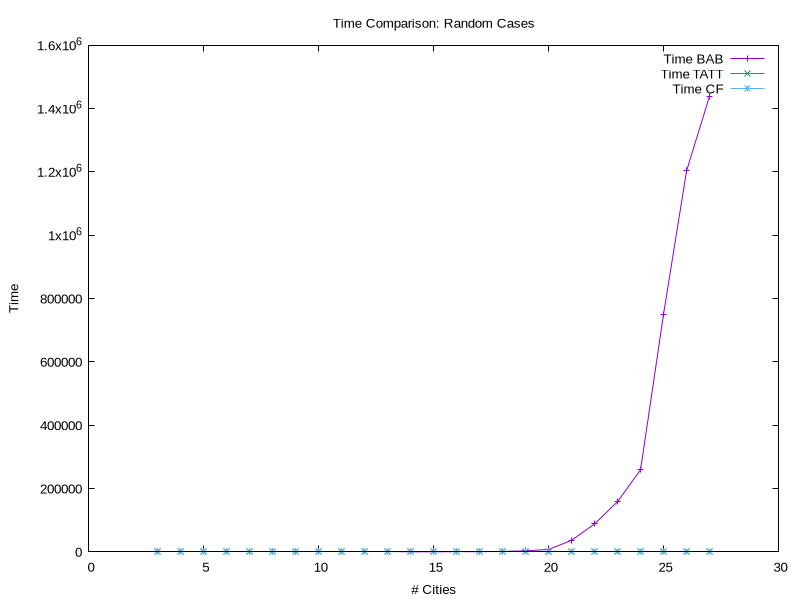
\includegraphics[width=0.9\textwidth]{random_plot_times.png}
\caption{Tempo de execução dos três algoritmos por tamanho do problema}
\label{fig:randomTimes}
\end{figure}

\begin{figure}
\centering
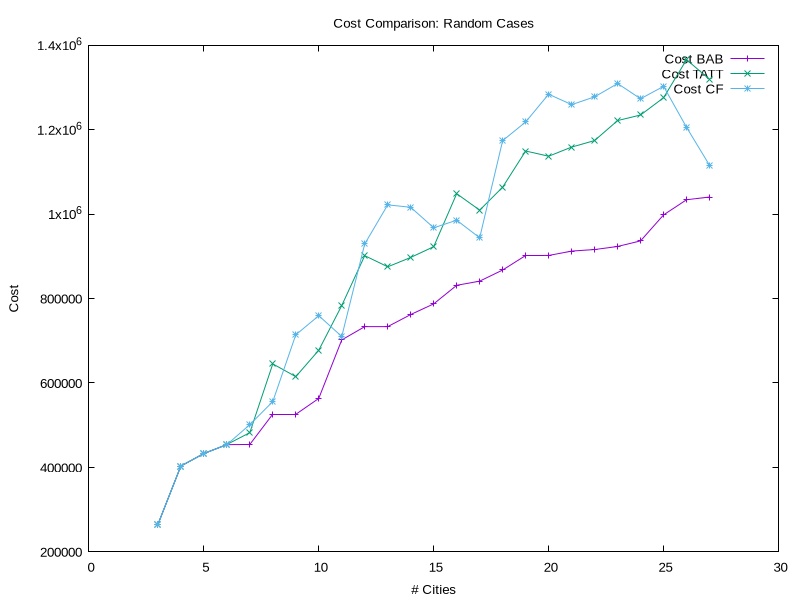
\includegraphics[width=0.9\textwidth]{random_plot_costs.png}
\caption{Custo das soluções dos três algoritmos por tamanho do problema}
\label{fig:randomCosts}
\end{figure}

Já no gráfico de custos das soluções (Figura~\ref{fig:randomCosts}), podemos
ver que o CF geralmente produz soluções melhores que o TATT, e que ambos
failham em encontrar a solução ótima, porém mantém um fator de aproximação
constante, não superando esse ponto.

\pagebreak

\subsection{Problemas da TSPLIB}
Os algoritmos também foram executados com os problemas de tipo euclideano 2D da TSPLIB
\cite{johnson1997traveling}.
Para os problemas da TSPLIB há mais cidades, por isso não foi possível executar
o algoritmo Branch and Bound nesses casos. Porém, os algoritmos aproximativos
foram executados bem rapidamente para esses casos, o que abriria a possibilidade
para refinar as soluções com buscas aleatórias e outras heurísticas de melhorias,
o que não foi feito nesse trabalho.

\begin{figure}
\centering
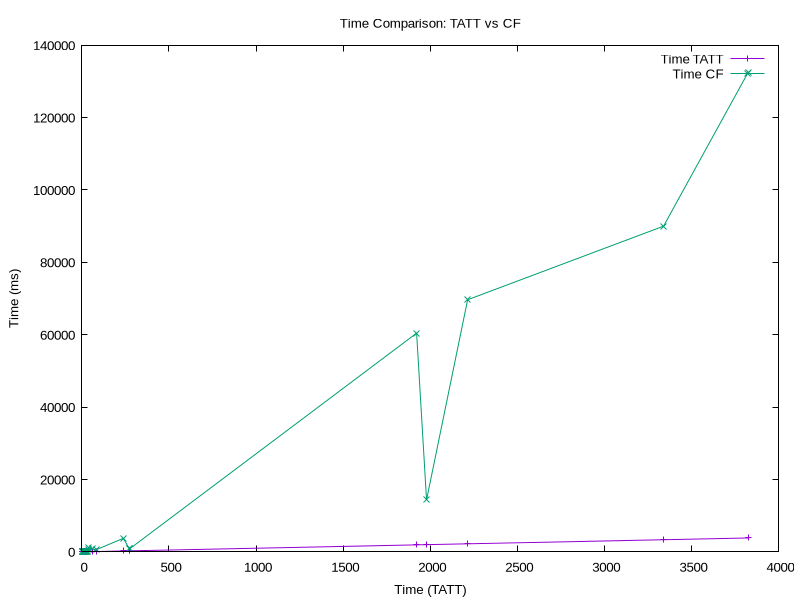
\includegraphics[width=0.9\textwidth]{tsplib_plot_times.png}
\caption{Tempo de execução dos algoritmos aproximativos por tempo}
\label{fig:tsplibTimes}
\end{figure}

Com relação aos tempos de execução (Figura~\ref{fig:tsplibTimes}), podemos ver os tempos de execução dos algoritmos
aproximativos e verificar que o Christofides possui um custo maior que o TATT.
Isso é facilmente explicado ao notar que o CF executa todos os passos do TATT:
criar a árvore geradora, fazer o Tour de Euler e obter o Circuito Hamiltoniano,
então fechá-lo, mas o CF também faz o uso de emparelhamentos mínimos. Em nossa
implementação, foi usado o algoritmo de Blossom, que é $O(|E||V|^2)$, e facilmente
supera a complexidade $O(|V|^2)$ do TATT.

Já com relação aos custos das soluções geradas, vemos que o CF é capaz de gerar
soluções melhores consistentemente, porém não chegam a ser $2/3$ do custo das
soluções do TATT como o pior caso sugere. O caso médio é diferente.

\begin{figure}
\centering
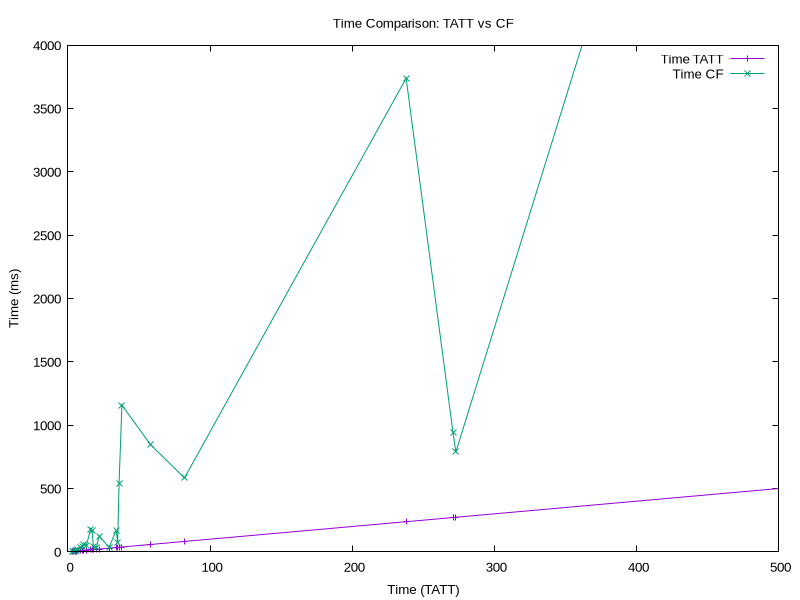
\includegraphics[width=0.9\textwidth]{tsplib_plot_times_zoom.png}
\caption{Tempo de execução dos algoritmos aproximativos por tempo (Zoom)}
\label{fig:tsplibTimesZoom}
\end{figure}

\begin{figure}
\centering
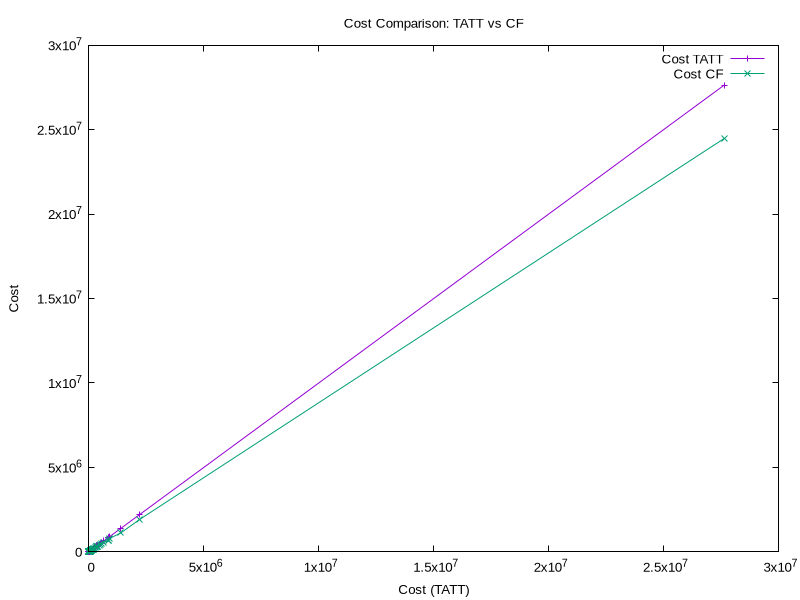
\includegraphics[width=0.9\textwidth]{tsplib_plot_costs.png}
\caption{Custo das soluções dos algoritmos aproximativos por tempo}
\label{fig:tsplibCosts}
\end{figure}

\begin{figure}
\centering
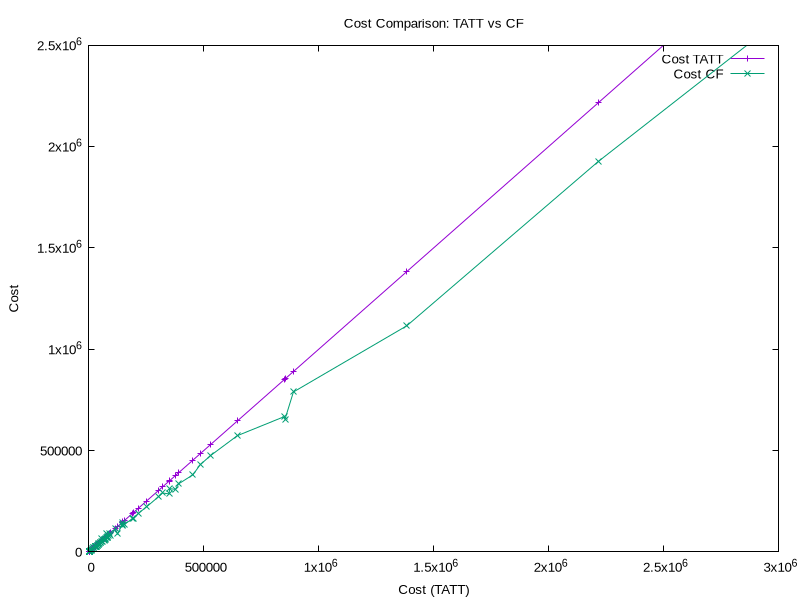
\includegraphics[width=0.9\textwidth]{tsplib_plot_costs_zoom.png}
\caption{Custo das soluções dos algoritmos aproximativos por tempo (Zoom)}
\label{fig:tsplibCostsZoom}
\end{figure}

Por fim, ao observar os fatores de aproximação, usando os dados fornecidos pela
TSPLIB e comparando com nossa implementação (Figura~\ref{fig:tspApproxFactors}),
nós observamos que o CF realmente respeita um fator de $O(3/2)$, e o TATT respeita
o fator de $O(2)$, com um caso médio semelhante entre os dois.

\begin{figure}
\centering
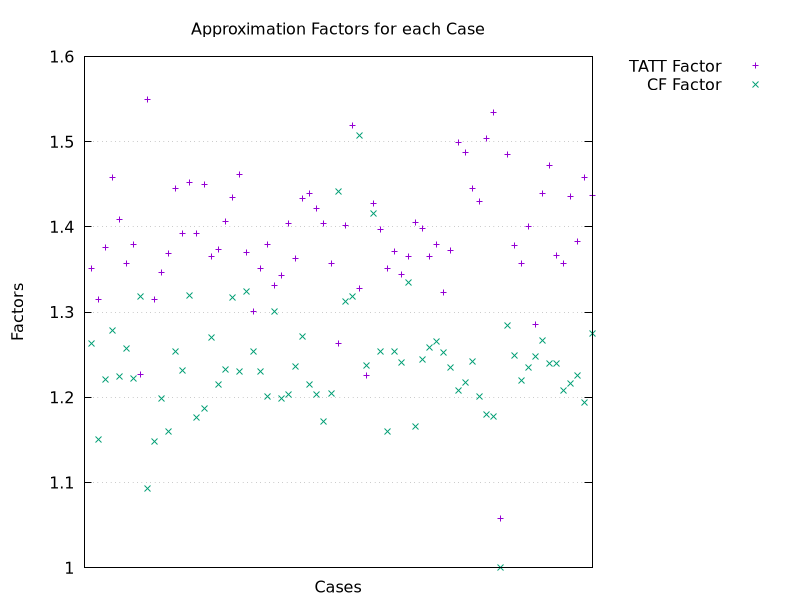
\includegraphics[width=0.9\textwidth]{factors.png}
\caption{Fatores de Aproximação dos algoritmos aproximativos}
\label{fig:tspApproxFactors}
\end{figure}

\pagebreak

\section{Conclusões}
Como os algoritmos diferem em tempo de execução e qualidade das soluções, eles
são úteis para casos diferentes \cite{lawler1985traveling}.
Pelo tempo de execução dos algoritmos, o TATT
pode ser a melhor opção para tarefas que precisem de resultados rápidos,
como unidades em jogos que precisem de calcular sua rota frequentemente,
enquanto o CF pode ser a melhor opção para tarefas comuns e diárias, e o
Branch and Bound a melhor opção para tarefas de alto risco que tenham um tempo
de planejamento maior, onde é possível esperar dias por uma solução.

\bibliographystyle{sbc}
\bibliography{tsp}

\end{document}
